% LaTeX Workshop: Build with recipe, latextmk
% compilation sequence
% pdflatex Draft.tex
% bibtex Draft
% pdflatex Draft.tex
% pdflatex Draft.tex


\documentclass[12pt,a4paper]{article}

% Essential packages
\usepackage[utf8]{inputenc}
\usepackage[T1]{fontenc}
\usepackage{amsmath,amsfonts,amssymb}
\usepackage{graphicx}
\usepackage{float}
\usepackage{url}
\usepackage{hyperref}
\usepackage{geometry}
\usepackage{setspace}
\usepackage{titlesec}
\usepackage{caption}
\usepackage{subcaption}
\usepackage{booktabs}
\usepackage{siunitx}
\usepackage{lineno}
\usepackage{natbib}
\usepackage{multirow}
\usepackage{pdflscape}

%to add the prime symbols to arcim and arcsec coordinates
\usepackage{textcomp}
\newcommand{\arcmin}{\ensuremath{^{\prime}}}
\newcommand{\arcsec}{\ensuremath{^{\prime\prime}}}

% Page setup
\geometry{
    a4paper,
    margin=2.5cm,
    top=3cm,
    bottom=3cm
}

% Line spacing
\doublespacing

% Line numbers (uncomment if required by journal)
% \linenumbers

% Section formatting
\titleformat{\section}{\large\bfseries}{\thesection.}{1em}{}
\titleformat{\subsection}{\normalsize\bfseries}{\thesubsection.}{1em}{}

% Figure and table captions
\captionsetup{font=small,labelfont=bf}

% Hyperlink setup
\hypersetup{
    colorlinks=true,
    linkcolor=black,
    citecolor=blue,
    urlcolor=blue
}

% Title page information
\title{\textbf{The impact of forest management on the temperature sensitivity of SOC decomposition in european forests}}

\author{
    Lorenzo Menichetti\textsuperscript{1,2}*, 
    Second Author\textsuperscript{1}, 
    Third Author\textsuperscript{3}\\
    Etc.\textsuperscript{3}\\
    \\
    \textsuperscript{1}Natural Resources Institute Finland (LUKE), \\
    \hspace*{0.5cm}Latokartanonkaari 9 00790 Helsinki, Finland\\
    \textsuperscript{2}Swedish University of Agricultural Sciences (SLU), \\
    \hspace*{0.5cm}Inst för Ekologi, Box 7044 750 07 Uppsala, Sweden\\
    \textsuperscript{3}[Third Institution]\\
    \\
    *Corresponding author: \href{mailto:Lorenzo.Menichetti@luke.fi}{Lorenzo.Menichetti@luke.fi}
}

\date{}

\begin{document}

\maketitle

\begin{abstract}
\noindent
\textbf{Background:} Provide context and rationale for your study. Briefly explain the problem or gap in knowledge that your research addresses.

\textbf{Methods:} Summarize your experimental design, key methods, and analytical approaches used in the study.

\textbf{Results:} Present the main findings of your research, including key quantitative results and statistical significance where applicable.

\textbf{Conclusions:} State the main conclusions and their broader implications. Highlight the significance of your findings and potential applications.

\textbf{Keywords:} keyword1, keyword2, keyword3, keyword4, keyword5
\end{abstract}

\newpage

\section{Introduction}


\subsection{Background and Rationale}


\subsection{Objectives and Hypotheses}

Clearly state your research objectives and hypotheses. For example:
\begin{itemize}
    \item \textbf{Primary objective:} To investigate the relationship between X and Y
    \item \textbf{Secondary objectives:} To evaluate Z and assess W
    \item \textbf{Hypothesis:} We hypothesize that X will significantly affect Y under conditions Z
\end{itemize}






\section{Materials and Methods}

\subsection{Holisoils project introduction}

HoliSoils - Holistic management practices, modelling and monitoring for European forest soils, is an EU funded project (Horizon 2020, Grant Agreements number 101000289), completed in October 2026, with the main aim to develop a harmonised soil monitoring framework.\\
More specifically, the project aimed at developing a consistent knowledge framework of  soil properties, processes, biodiversity and soil microbiota activity, in connection with soil-based ecosystem services (wood production, reduction of greenhouse gas emissions, water supply, soil nutrient retention, avoidance of land degradation), particularly in connection with different management approaches.
Modeling was another of the focuses, specifically improving current models and harmonise them into a monitoring framework for estimating ecosystem fluxes. Directly connected with the modeling activity, the project developed a set of standardised sampling and monitoring protocols shared among all actors for greenhouse gas (GHG) reporting. These were used across multiple sampling campaigns across three consecutive years in different locations over Europe, and results have been collected in a comprehensive database of GHG measurements together with additional edaphic and ecological variables.

\subsubsection{Actors and nations involved}
The project involved a consortium of 20 project partners, 18 from EU and partners from South America (Uruguay) and Asia (Japan):
\begin{itemize}
\item Natural Resources Institute Finland (Luonnonvarakeskus), Luke, Finland
\item Institute of Microbiology of the Czech Academy of Sciences (Mikrobiologický ústav AV ČR, v. v. i.), IMIC, Czech Republic
\item French National Centre for Scientific Research (Centre National de la Recherche Scientifique Research institute), CNRS, France
\item Johann Heinrich von Thünen Institute (Johann Heinrich von Thünen-Institut Research institute), TI, Germany
\item Basque Centre for Climate Change (Asociacion BC3 Basque Centre for Climate Change Klima Aldaketa Ikergai), BC3, Spain
\item Vrije University Amsterdam (Stichting VU University), VU, Netherlands
\item European Forest Institute, EFI, Finland
\item Wageningen Research Foundation (Stichting Wageningen), WR, Netherlands
\item International Soil Reference \& Information Centre (Stichting International Soil Reference \& Information Centre), ISRIC, Netherlands
\item Stockholm University (Stockholms Universitet), SU, Sweden
\item Transylvania University of Brașov (Universitatea Transilvania din Brașov), UTBV, Romania
\item University of Barcelona (Universitat de Barcelona), UB, Spain
\item University of Aberdeen (The University Court of The University of Aberdeen), UNIABDN, UK
\item Vytautas Magnus University (Vytauto Didziojo universitetas), VMU, Lithuania
\item Aix-Marseille University (Aix-Marseille Université), AMU, France
\item Technical University of Munich (Technische Universität München), TUM, Germany
\item Technical University in Zvolen (Technick\'{a} univerzita vo Zvolene), TUZVO, Slovakia
\item Forest Science \& Technology Centre of Catalonia (Centre de Ciència i Tecnologia Forestal de Catalunya), CTFC, Spain
\item National Institute for Agricultural Research (Instituto Nacional de Investigación Agropecuaria), INIA, Uruguay
\item Forestry \& Forest Products Research Institute, FFPRI, Japan
\end{itemize}


\subsubsection{The greenhouse gas management effort and how it connects to other parts of the project}




\subsection{Sites and study design}
\begin{landscape}
\begin{table}[htbp]
\centering
\caption{Summary of study sites}
\label{tab:study_sites}
\footnotesize
\begin{tabular}{p{2.1cm}p{2.2cm}p{2.5cm}p{2.2cm}p{2.8cm}p{2.6cm}p{3.2cm}}
\toprule
\textbf{Country} & \textbf{Site} & \textbf{Coordinates} & \textbf{Climate} & \textbf{Dominant Species} & \textbf{Soil Type} & \textbf{Treatments} \\
\midrule
\multirow{2}{*}{\textbf{Finland}} 
& Karstula & 62\textdegree54\arcmin43.343\arcsec N; 24\textdegree34\arcmin16.021\arcsec E & Boreal & Scots pine & Sandy loam & Long-term fertilization (1950s) \\
& Ränskälänkorpi & 61\textdegree11\arcmin N, 25\textdegree16\arcmin E & Boreal & Norway spruce & Drained peatland & Control, clear-cut, selection harvest \\
\midrule
\textbf{Germany} & Kranzberg & 48\textdegree25\arcmin8.4\arcsec N; 11\textdegree39\arcmin39.6\arcsec E & Continental (Dfb) & Norway spruce / Mixed spruce-beech & Cambisols, luvisols & Precipitation gradient, drought legacy \\
& Kalheim & 11\textdegree49'19.2''E; 48\textdegree56'8.16''N & Continental (Dfb) & Norway spruce / Mixed spruce-beech & Terra fusca-cambisol & Precipitation gradient, drought legacy \\
& Wasserburg & 12\textdegree04'22.8''E; 48\textdegree08'31.2''N & Continental (Dfb) & Norway spruce / Mixed spruce-beech & Cambisols, luvisols & Precipitation gradient, drought legacy \\
\midrule
\multirow{3}{*}{\textbf{Netherlands}} 
& Kroondomein & 52\textdegree12\arcmin18.17\arcsec N; 5\textdegree51\arcmin54.47\arcsec E & Maritime (Cfb) & Scots pine & Poor sandy (Albic Podzol) & Control, high-thinning, shelterwood, clearcut \\
& Zwolse Bos & 52\textdegree25\arcmin14.41\arcsec N; 6\textdegree2\arcmin3.67\arcsec E & Maritime (Cfb) & Scots pine & Poor sandy (Albic Podzol) & Control, thinning (9\%), shelterwood (61\%), clearcut (100\%) \\
& Hoge Veluwe & 52\textdegree5\arcmin23.95\arcsec N; 5\textdegree48\arcmin14.68\arcsec E & Maritime (Cfb) & Scots pine & Poor sandy (Dystric Cambisol) & Same 4 treatments as above \\
\midrule
\multirow{2}{*}{\textbf{France}} 
& St. Mitre & 43\textdegree27\arcmin0\arcsec N; 5\textdegree2\arcmin24\arcsec E & Mediterranean (Csa) & Aleppo pine & Sandy loamy calcareous & Thinning intensity $\times$ understory management \\
& St. Christol & 44\textdegree02\arcmin58.0\arcsec N 5\textdegree32\arcmin35.8\arcsec E & Mediterranean (Csa) & \textit{Quercus pubescens} & Calcisol & Control, CD50$\pm$Slash, CD100$\pm$Slash \\
\midrule
\multirow{2}{*}{\textbf{Spain}} 
& Gamiz & 42\textdegree49\arcmin2.32\arcsec N; 2\textdegree37\arcmin10.67\arcsec W & Oceanic (Cfb) & \textit{Quercus faginea} & Clay loam Luvisol & Control, CD50$\pm$Slash, CD100$\pm$Slash \\
& Llobera & 41\textdegree57\arcmin08\arcsec N; 1\textdegree27\arcmin55\arcsec E & Sub-Mediterranean & Black pine (\textit{P. nigra}) & Lithic or Typic Xerorthent & Light/heavy thinning $\pm$ prescribed burning \\
& Secanella & 41\textdegree56'16''N; 1\textdegree26'05''E & Sub-Mediterranean & Black pine (\textit{P. nigra}) & Lithic or Typic Xerorthent & Light/heavy thinning $\pm$ prescribed burning \\
\midrule
\textbf{Slovakia} & Dobroc & 48\textdegree40'24.6''N; 19\textdegree40'44.4''E & Continental (Dfb) & Norway spruce / Mixed forest & Dystric Cambisol & Monoculture vs mixed stand \\
\midrule
\textbf{Romania} & Dumbravita & 45\textdegree46\arcmin10.0\arcsec N; 25\textdegree28\arcmin26.0\arcsec E & Continental (Dfb) & \textit{Quercus robur} & Cambisol & Control, CD50$\pm$Slash, CD100$\pm$Slash \\
\bottomrule
\end{tabular}
\end{table}
\end{landscape}

\textbf{Treatment abbreviations:}
CD50/CD100: 50\%/100\% canopy removal; $\pm$Slash: with/without logging residue management; BA: Basal area reduction percentage

\subsubsection{Finland}
\paragraph{Karstula}
Long-term fertilization experiment site established in late 1950s by Finnish Forest Research Institute in Scots pine forest on sandy loam soils.
\paragraph{Ränskälänkorpi}
Norway spruce site on drained peatland with control, clear-cut, and selection harvest areas. CO2 flux measurements using eddy covariance towers and automatic chambers with continuous soil temperature and moisture monitoring.

\subsubsection{Germany}
\paragraph{Kranzberg}
Precipitation gradient study across three locations in Bavaria evaluating mature Norway spruce stands compared to mixed spruce-beech stands on Cambisols and Luvisols. Soil respiration (Rs) and heterotrophic respiration (Rh) measured biweekly during 2022-2023 vegetation periods with continuous soil temperature and moisture monitoring. Includes drought legacy experiment examining long-term effects of extreme drought (2014-2018 rainfall exclusion).

\subsubsection{Netherlands}
Study across multiple sites investigating effects of forest management on soil respiration in Scots pine forests on poor sandy soils, with treatments established in February-March 2019.
\paragraph{Kroondomein} Soil CO2 flux measurements using EGM-5 analyzer with trenching for heterotrophic/autotrophic separation, continuous soil temperature and moisture monitoring with TOMST TMS-4 sensors.
\paragraph{Zwolse Bos} Identical experimental design to Kroondomein with four management treatments: control, high-thinning (9\% BA reduction), shelterwood (61\% BA reduction), and clearcut (100\% BA reduction).
\paragraph{Hoge Veluwe} Same four treatment design with biweekly CO2 measurements from May 2022-September 2024, continuous soil temperature and moisture monitoring.

\subsubsection{France}
\paragraph{St. Mitre} Mediterranean Aleppo pine forest on sandy loamy calcareous soils examining combined effects of thinning intensity and understory management. Established in 2007 with five treatments: intensive thinning with/without shrubs (I+, I-), moderate thinning with/without shrubs (M+, M-), and control (C). Monthly soil respiration measurements using EGM-5 CO2 analyzer with continuous microclimate monitoring using TOMST TMS-4 dataloggers.
\paragraph{St. Christol} Mediterranean site with Quercus pubescens monoculture on Calcisol soils. Experimental design established April 2022 with five treatments across four blocks: control, 50\% and 100\% canopy removal with/without slash treatments. Total 40 plots with continuous soil temperature and moisture monitoring.

\subsubsection{Spain}
\paragraph{Gamiz} Northern Spain site at 580m elevation in Quercus faginea dominated forest on clay loam Luvisol. Experimental design established October 2021 with five treatments across four blocks: control, 50\% and 100\% canopy removal with/without slash. Total 40 plots with continuous soil temperature and moisture monitoring.

\subsubsection{Slovakia}
\paragraph{Dobroc} Site at 950m elevation on Dystric Cambisol comparing 70-year-old Norway spruce monoculture with adjacent mixed forest (spruce, beech, silver fir). Root exclusion trenching to separate heterotrophic/autotrophic respiration, biweekly CO2 measurements since August 2021 using LI-COR LI-7810 with continuous soil temperature and moisture monitoring. Site affected by bark beetle outbreak in 2022 followed by clearcut in 2023.
\subsubsection{Romania}
\paragraph{Dumbravita} Eastern Romania site at 544m elevation in Quercus robur monoculture on Cambisol soils. Experimental treatments established March 2022 with five treatments across four blocks: control, CD50+/-Slash, CD100+/-Slash. Total 40 plots with continuous soil temperature and moisture monitoring.


\subsubsection{Sampling}

\paragraph{Trenching}
In most sites all treatments have both control and trenched subtreatments. The aim of the trenching is to remove all autotrophic respiration from the total soil respiration. Threnching areas were established (on an area of approximately 2 square meters) by digging trenches at a depth of approximately 30-40 cm and then placing root exclusion fabric around the trenched area. The fabric had around 50 $\mu$m mesh size, which prevents roots but allows mychorrizae to penetrate the area, as well as water.

\subsubsection{Sampling}
Soil CO$_2$ from control and trenched locations was measured approximately every second week with closed chambers and gas concentration analyzers (see \ref{par:devices}), basing the flux estimate on the linear regression of the concentration increase over time.
Measurement points for the soil chambers have been established with metal or plastic collars, or in some cases (organic soils) by installing the chamber deeper into the soil, to ensure that there was not air flow between the chamber and the atmosphere.

\paragraph{Devices}\label{par:devices}
ASK SITE OWNER!!!!!




\paragraph{Covariates}
Soil temperature and in some cases moisture have been recorded in the upper layer (5-10 cm) with various commercially available sensors.



\subsection{The database}

\subsubsection{Organization of the published dataset}
The database is published as a static resource on Zenodo (ADD LINK HERE!!!!!!!).

The dataset is structured in folders, each corresponding to one site. Inside each folder, there are subfolders corresponding to the measurement series. Each measurement series is a sampling campaign, during which each instrument was started and run for several samplings of multiple plots.
Inside each series subfolder there are Apache feather files corresponding to each single measurement. 
Apache Feather is an open columnar binary file format designed for fast data interchange between different programming languages, particularly Python and R. It provides efficient serialization and deserialization of dataframes with minimal overhead, 
which makes it ideal for storing a large number of relatively small files.\\

Each feather file, so each measurement, is associated to a line in the metadata file in each site folder. This contains also the respiration fluxes estimated automatically. The estimates were in some cases trimmed manually by the uploading operators, who selected the window in the time series on which to perform the regression to calculate the fluxes. In other cases, when the operator did not select a manual trimming window, the trimming was done automatically.
The metadata files are then collected together in one single general file in the root folder of the dataset (file "All\_sites.csv"), where the analyses in this study were performed.
The dataset is distributed with both calculated flux values and raw measurements in case the user of the database would want to develop own flux estimation approaches.


\subsubsection{Automatic trimming logic}
Jani to write this.

\subsubsection{Dataset fields and units}
A table here, to write together with Jani




\subsubsection{Descriptive analysis of the data}



\paragraph{Recoding of the treatments}


\subsection{Modeling SOC decomposition dependency on climate}


\subsection{The model}
Soil respiration was modeled as a function of temperature, moisture, and seasonal effects:
\begin{equation}
R = A \times \xi_{\text{temp}} \times \xi_{\text{moisture}} \times \xi_{\text{seasonal}} \times \lambda
\end{equation}

where $A$ represents baseline respiration rates (plot-specific), and the environmental multipliers are defined as follows:

\textbf{Temperature sensitivity} following Lloyd and Taylor kinetics with temperature sensitivity ($E_0$):
\begin{equation}
\xi_{\text{temp}} = \exp\left(-\frac{E_0}{(T + 273.15) - T_0}\right)
\end{equation}
where $T$ is temperature (°C) and $T_0 = 227.13$ K is a reference temperature constant.

\textbf{Moisture response} using a quadratic relationship:
\begin{equation}
\xi_{\text{moisture}} = aM - bM^2
\end{equation}
where $M$ is soil moisture content, and $a$ and $b$ are treatment-specific parameters controlling the shape of the moisture response curve.

\textbf{Seasonal variation} through a cosine function:
\begin{equation}
\xi_{\text{seasonal}} = \text{amplitude} \times \cos\left(\frac{2\pi}{365} \times \text{day\_year} + \frac{2\pi}{365} \times (\text{peak\_day} - 1) - \frac{\pi}{2}\right)
\end{equation}
where day\_year is the day of the year (1-365), peak\_day defines the timing of maximum seasonal effect, and amplitude controls the magnitude of seasonal variation.

\textbf{Trenching effect} distinguishing trenched from non-trenched plots:
\begin{equation}
\lambda = \begin{cases}
1 & \text{if trenched} \\
\text{linear\_mult} & \text{if not trenched}
\end{cases}
\end{equation}
where linear\_mult represents the multiplicative effect of root presence in non-trenched plots.

\subsection{The Bayesian framework}
Due to the computational requirements of the calibration, we employed a two-stage Bayesian inference approach to ensure robust parameter estimation and easier convergence. The procedure consisted of an initial calibration phase to identify the best starting value (to speed up convergence) followed by full MCMC sampling.


\subsubsection{MCMC initialization and sampling}
Prior to MCMC sampling, we obtained maximum a posteriori (MAP) parameter estimates using stochastic variational inference (SVI) implemented in NumPyro. This pre-estimation step provides good starting values for the MCMC chains, reduces burn-in time, and helps identify potential convergence issues before computationally expensive full sampling.
The SVI approach uses an AutoNormal guide, which assumes a mean-field variational approximation where each parameter is independently normally distributed. This approximation, while simpler than the true posterior, provides a computationally efficient way to locate the posterior mode that will be later used for initializing the MCMC chains. The optimization was performed using the Adam optimizer with a learning rate of 0.01, running for 3,000 iterations to ensure convergence of the variational parameters.
Using the MAP estimates from SVI, we initialized 24 parallel MCMC chains by adding small random perturbations (noise scale = 0.05) around the MAP values. This initialization strategy, known as "jittering," ensures that chains start from different but reasonable locations in parameter space, facilitating better exploration of the posterior distribution while avoiding poor local optima that can occur with random initialization.
The MCMC sampling employed the No-U-Turn Sampler (NUTS) algorithm \citep{hoffman2014nuts}. NUTS is particularly well-suited for high-dimensional problems like our hierarchical model, as it can efficiently navigate complex posterior geometries. We configured NUTS with a target acceptance probability of 0.9.
Each chain was run for 20,000 iterations total: 5,000 warmup samples, followed by 15,000 retained samples for posterior inference. The warmup phase allows NUTS to learn the local geometry of the posterior distribution, which is crucial for efficient sampling in subsequent iterations. The parallel chain approach enables both computational efficiency (especially in our case, run on a highly parallelized cluster, see Section~\ref{sec:implementation}) and robust convergence diagnostics through between-chain comparisons.

\subsubsection{Prior distributions}
Prior distributions were informed by ecological knowledge and previous studies:
\begin{align}
E_0 &\sim \mathcal{N}(398.5, 20^2) && \text{(activation energies typical for soil processes)} \\
A &\sim \mathcal{N}(400, 50^2) && \text{(baseline respiration rates)} \\
a &\sim \mathcal{N}(3.11, 1^2) && \text{(moisture response parameters)} \\
b &\sim \mathcal{N}(2.42, 1^2) && \text{(based on soil-water relationships)} \\
\text{amplitude} &\sim \mathcal{N}(0, 1^2) && \text{(seasonal variation magnitude)} \\
\text{peak\_day} &\sim \mathcal{N}(196, 10^2) && \text{(mid-growing season timing)} \\
\text{linear\_mult} &\sim \mathcal{N}(1, 0.5^2) && \text{(trenching effect multiplier)} \\
\sigma &\sim \text{Exp}(1) && \text{(observation error)}
\end{align}

\subsubsection{Likelihood}
The likelihood function assumes that observed respiration measurements follow a normal distribution around the model predictions:
\begin{equation}
R_{\text{obs},i} \sim \mathcal{N}(R_{\text{pred},i}, \sigma^2)
\end{equation}
where $R_{\text{obs},i}$ is the $i$-th observed respiration measurement, $R_{\text{pred},i}$ is the corresponding model prediction, and $\sigma$ represents the standard deviation of observation errors. This formulation accounts for measurement uncertainty and natural variability not captured by the environmental predictors, with the assumption that residuals are normally distributed and homoscedastic across the range of predicted values.

\subsubsection{Sampling stratification}
The model sampling relied on stratification to ensure proper inference across the huge variety of treatments. Our sampling design incorporated three levels of stratification:

\textbf{Treatment level:} The model accounts for treatment-specific parameters ($E_a$, $a$, $b$, amplitude, peak\_day) that capture systematic differences in respiration responses between experimental treatments. This allows for treatment-specific temperature sensitivities, moisture responses, and seasonal patterns, based on the assumption that treatments will influence decomposition kinetics.

\textbf{Plot level:} Baseline respiration rates ($A$) were modeled as plot-specific parameters to account for spatial heterogeneity in soil properties, microbial communities, and other plot-level factors not explicitly measured. This approach recognizes that plots within the same treatment may have different inherent respiration capacities due to local environmental conditions. The most important plot-level source of variation we expect is substrate amount, meaning C stocks, and possibly local substrate quality.

\textbf{Observation level:} Individual respiration measurements were treated as independent observations conditional on the plot and treatment effects, with measurement error captured through the likelihood function. This level accounts for temporal variation within plots and measurement uncertainty.

Treatment effects are estimated by pooling information across all plots within each treatment, while plot-level heterogeneity is explicitly modeled rather than ignored. This stratification ensures that statistical inference properly reflects the experimental design and sampling structure of the study.


\subsection{Missing Values Imputation Approach}
Due to sampling issues and diversity of the sampling approaches between sites, our dataset contained missing values for soil temperature (18.5\% of observations) and particumarly soil moisture (41.8\% of observations). Rather than using traditional approaches like mean imputation or listwise deletion, which can introduce bias or reduce statistical power, or dropping completely the moisture function discarding some available information, we implemented a hierarchical Bayesian missing data model that accounts for site-specific patterns while properly propagating uncertainty.
Due to computational constraints, missing values were modeled using site-level parameters, assuming that temperature and moisture are relatively constant within a same site:soil moisture followed $M_{\text{mean},s} \sim \text{Beta}(2,2)$ scaled to $[0.1, 0.9]$ and temperature followed $T_{\text{mean},s} \sim \text{Normal}(15, 10)$, where $s$ indexes monitoring sites.
Missing observations were then imputed from their corresponding site-specific distributions within the main Bayesian model, ensuring uncertainty propagation through all parameter estimates. This approach reduced the missing data parameter space from potentially thousands of individual parameters to 4 parameters per site (N = Z sites), resulting in substantial computational efficiency gains while maintaining biological realism and proper uncertainty quantification. A model imputing missing values independently for each value would of course be more accurate in theory, but would imply an unfeasible number of Bayesian parameters in the model (many thousands) with consequent prohibitive memory and power requirements.



\subsection{Implementation and hardware}\label{sec:implementation}

All analyses were conducted in Python using JAX for numerical computing and NumPyro for Bayesian inference \citep{phan2019composable}. Computations were performed on the Puhti supercomputer cluster operated by CSC - IT Center for Science, Finland. The model was run on CPU nodes with 25 parallel processing cores allocated per job to ensure computational efficiency and optimal resource utilization within the high-performance computing environment.

Convergence was assessed through visual inspection of trace plots and Gelman-Rubin convergence diagnostic ($\hat{R}$) \citep{gelman1992inference, vehtari2021rank}. By implementing the sampling with a high number of parallel chains we allowed for robust convergence diagnostics by comparing results across independent chains.

Model outputs provided posterior distributions for all parameters, enabling quantification of uncertainty in treatment effects and environmental sensitivities. The high-performance computing infrastructure enabled extensive sampling (15,000 samples $\times$ 24 chains) necessary for reliable posterior inference in this complex hierarchical model.


\section{Results}

\subsection{Descriptive analysis}

\subsubsection{Soil respiration and temperature}
% CO2 vs temperature
\begin{figure}[H]
    \centering
    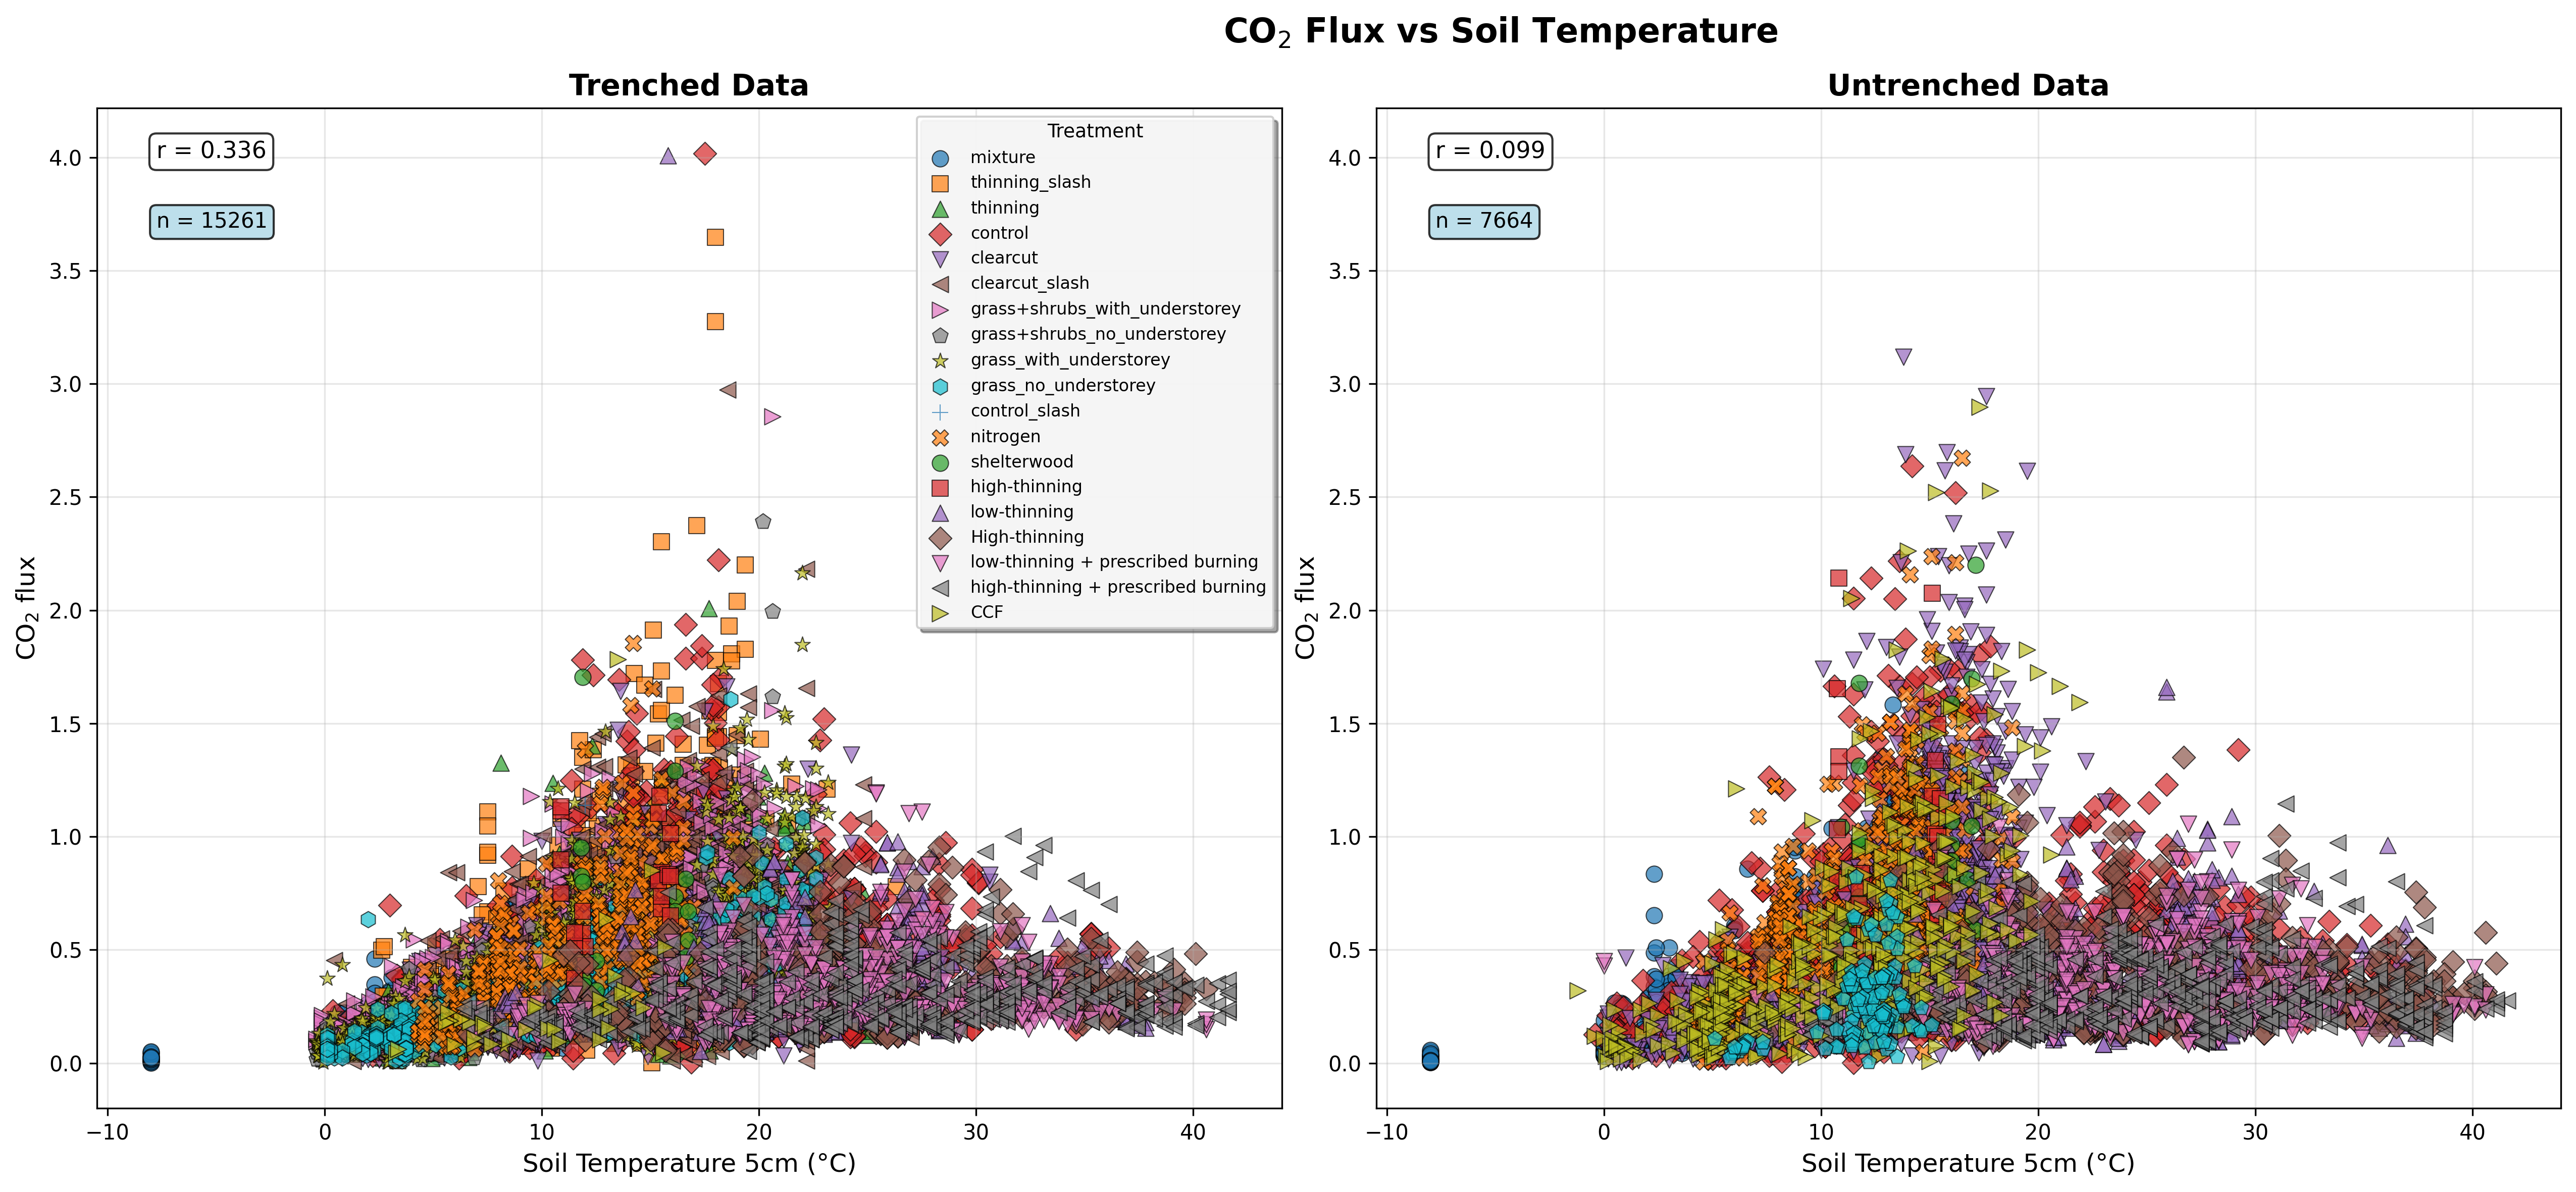
\includegraphics[width=0.8\textwidth]{"../co2_flux_temperature_comparison.png"}
    \caption{Example figure caption. Describe what the figure shows, including experimental conditions, sample sizes, and statistical tests. Error bars represent standard error of the mean. *p < 0.05, **p < 0.01.}
    \label{fig:co2_temp}
\end{figure}

\subsubsection{Soil respiration and moisture}
% CO2 vs tmoisture
\begin{figure}[H]
    \centering
    \includegraphics[width=0.8\textwidth]{"../co2_flux_moisture_comparison.png"}
    \caption{Example figure caption. Describe what the figure shows, including experimental conditions, sample sizes, and statistical tests. Error bars represent standard error of the mean. *p < 0.05, **p < 0.01.}
    \label{fig:co2_moisture}
\end{figure}

\subsubsection{Moisture and temperature interactions}
% temperature vs tmoisture
\begin{figure}[H]
    \centering
    \includegraphics[width=0.8\textwidth]{"../soil_temperature_moisture_comparison.png"}
    \caption{Example figure caption. Describe what the figure shows, including experimental conditions, sample sizes, and statistical tests. Error bars represent standard error of the mean. *p < 0.05, **p < 0.01.}
    \label{fig:temp_moisture}
\end{figure}


\subsubsection{Autotrophic and heterotrophic fluxes}

\subsubsection{Fluxes over time}
% Time series
\begin{figure}[H]
    \centering
    \includegraphics[width=0.8\textwidth]{"../co2_flux_timeseries.png"}
    \caption{Example figure caption. Describe what the figure shows, including experimental conditions, sample sizes, and statistical tests. Error bars represent standard error of the mean. *p < 0.05, **p < 0.01.}
    \label{fig:timeseries}
\end{figure}




\subsubsection{Modeling analysis}

% Model predictions
\begin{figure}[H]
    \centering
    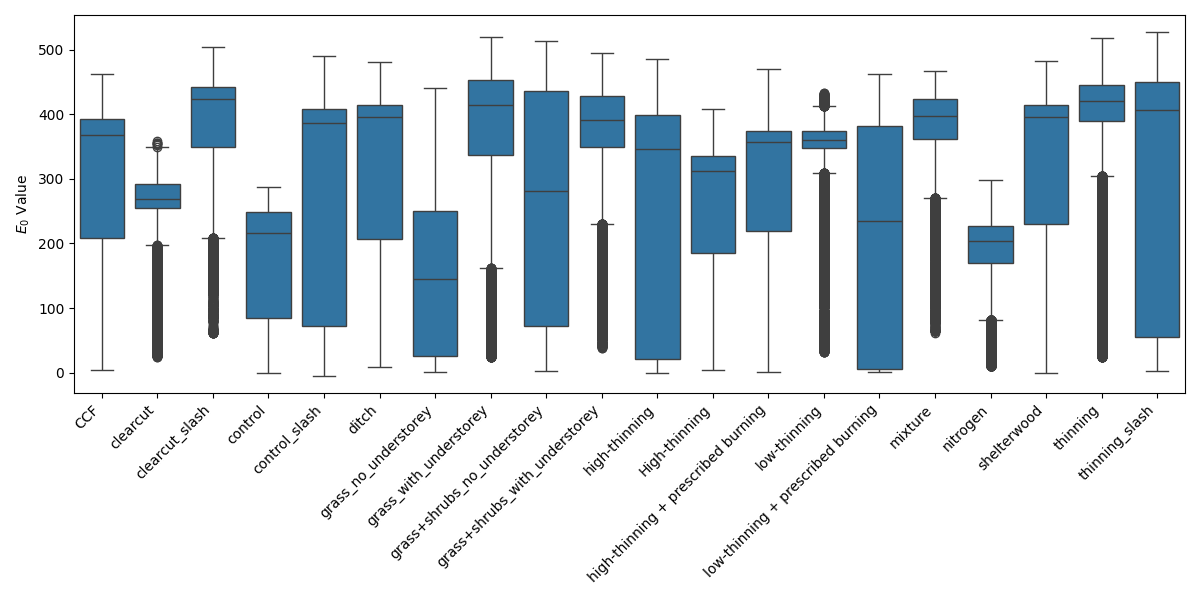
\includegraphics[width=0.8\textwidth]{"../ea_boxplot.png"}
    \caption{Model predictions here}
    \label{fig:model_fit}
\end{figure}

% E_0 parameter
\begin{figure}[H]
    \centering
    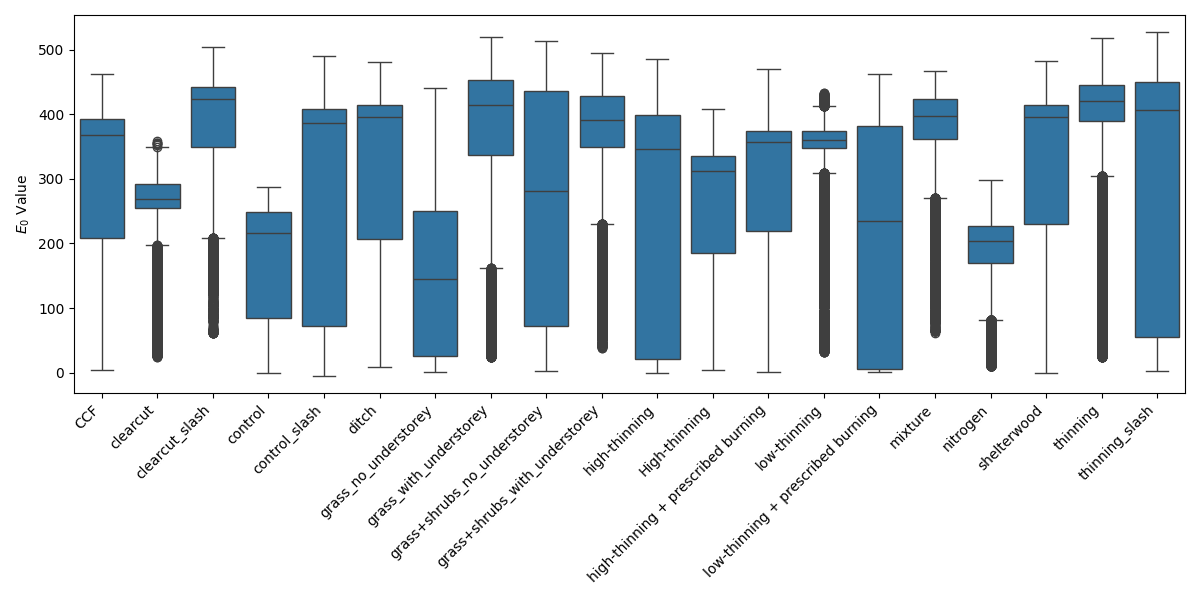
\includegraphics[width=0.8\textwidth]{"../ea_boxplot.png"}
    \caption{Example figure caption. Describe what the figure shows, including experimental conditions, sample sizes, and statistical tests. Error bars represent standard error of the mean. *p < 0.05, **p < 0.01.}
    \label{fig:ea_boxplot}
\end{figure}

\begin{figure}[H]
    \centering
    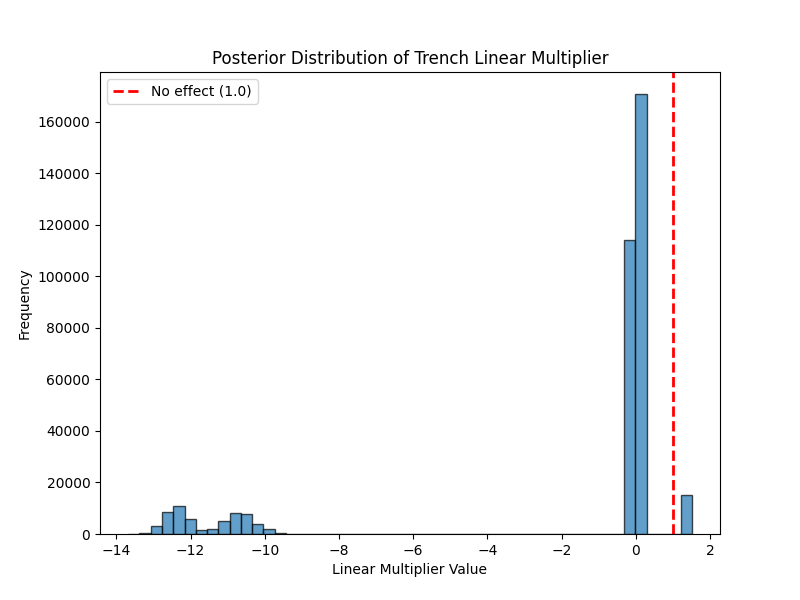
\includegraphics[width=0.8\textwidth]{"../linear_multiplier.png"}
    \caption{Example figure caption. Describe what the figure shows, including experimental conditions, sample sizes, and statistical tests. Error bars represent standard error of the mean. *p < 0.05, **p < 0.01.}
    \label{fig:linear_mult}
\end{figure}


% Other model params (except A)
\begin{figure}[H]
    \centering
    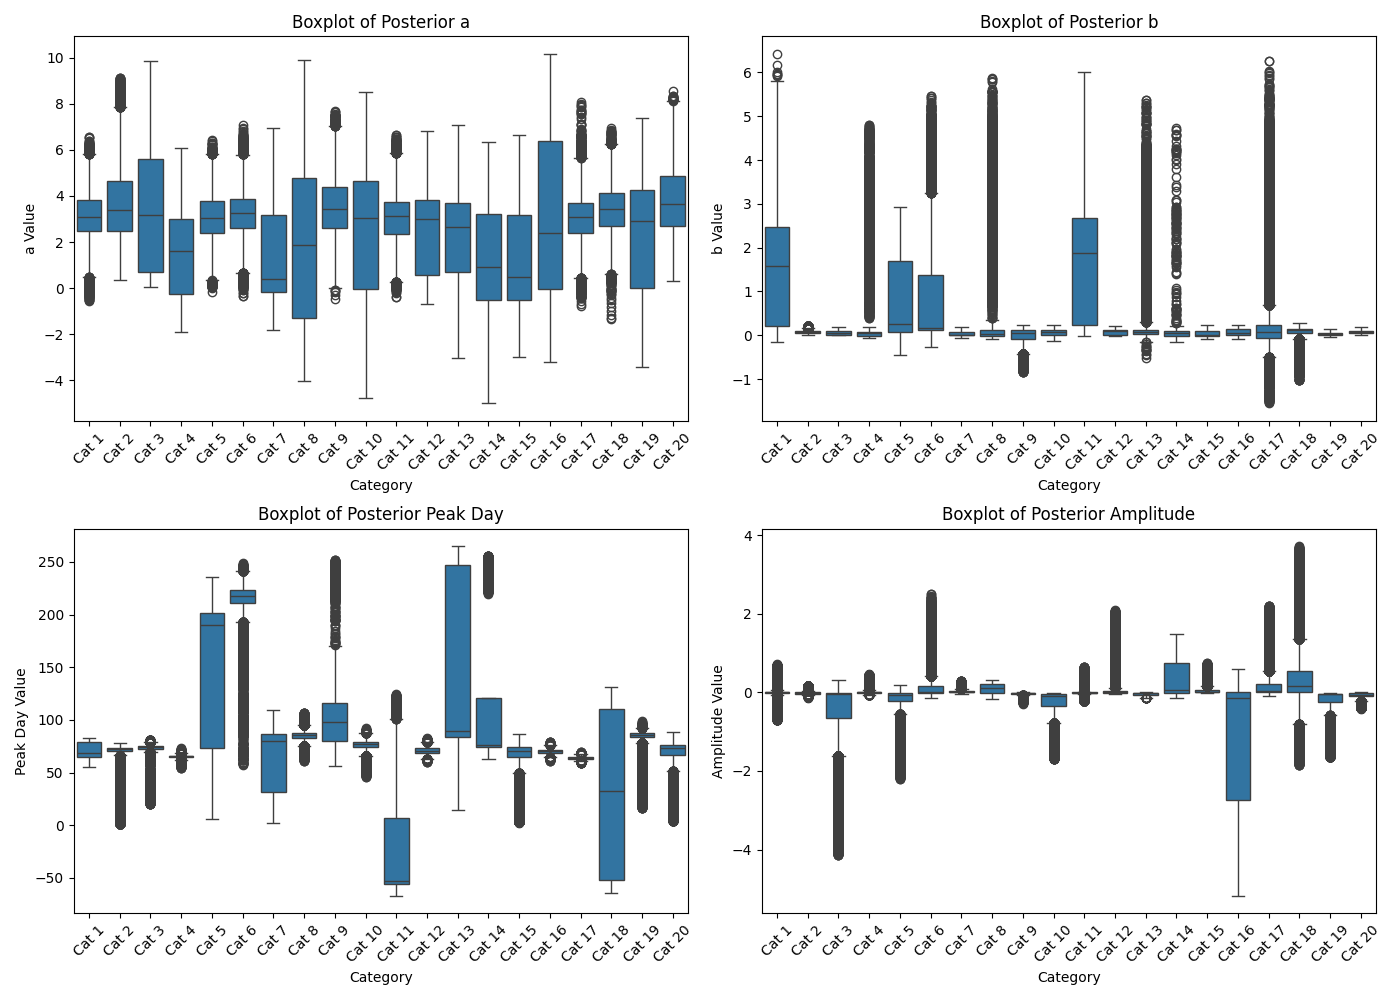
\includegraphics[width=0.8\textwidth]{"../other_params.png"}
    \caption{Example figure caption. Describe what the figure shows, including experimental conditions, sample sizes, and statistical tests. Error bars represent standard error of the mean. *p < 0.05, **p < 0.01.}
    \label{fig:other_params}
\end{figure}



\section{Discussion}

\subsection{Interpretation of Results}


\subsection{Limitations}

\subsubsection{Data limitations}

\paragraph{Mositure data}


\paragraph{Temperature data}
Netherlands measured only with TOMST at 10 cm depth



\subsubsection{Model limitations}


\subsection{Implications and Future Directions}



\section{Conclusions}

Summarize the key findings and their significance. Avoid simply repeating the abstract; instead, provide a synthesis that emphasizes the contribution of your work to the field.


\section*{Acknowledgments}

Acknowledge funding sources, institutional support, and individuals who contributed to the work but are not listed as authors.


\section*{Funding}

This work was supported by [Grant Agency] under Grant [Number]. [Author Name] was supported by [Fellowship/Scholarship].


\section*{Conflicts of Interest}

The authors declare no conflicts of interest.


\section*{Data and Code Availability}

The data that support the findings of this study are available as Open Data . . .

The code used for this analysis is available (for repeatability purposes, but the code is specific to the cluster we run it onto and needs some adaptation to run on other machines) at \url{https://github.com/ilmenichetti/Holisoils_fitting}





% Bibliography
\bibliographystyle{plain}
\bibliography{library}


\end{document}